\documentclass[Journal,letterpaper,BackFigs]{ascelike-new}
%% Please choose the appropriate document class option:
% "Journal" produces double-spaced manuscripts for ASCE journals.
% "NewProceedings" produces single-spaced manuscripts for ASCE conference proceedings.
% "Proceedings" produces older-style single-spaced manuscripts for ASCE conference proceedings. 
%
%% For more details and options, please see the notes in the ascelike-new.cls file.

% Some useful packages...
\usepackage[utf8]{inputenc}
\usepackage[T1]{fontenc}
\usepackage{lmodern}
\usepackage{graphicx}
\usepackage[figurename=Fig.,labelfont=bf,labelsep=period]{caption}
\usepackage{subcaption}
\usepackage{amsmath}
\usepackage{tabularx}
%\usepackage{amsfonts}
%\usepackage{amssymb}
%\usepackage{amsbsy}
\usepackage{newtxtext,newtxmath}
\usepackage[colorlinks=true,citecolor=red,linkcolor=black]{hyperref}
\newcommand{\Muste}[1]{}
%
% Please add the first author's last name here for the footer:
\NameTag{Banjavcic, \today}
% Note that this is not displayed if the NoPageNumbers option is used
% in the documentclass declaration.
%



\begin{document}

% You will need to make the title all-caps
\title{Spatial Uncertainty in Depth-Averaged Velocity and Discharge Determined from Stationary, Transect, and Longitudinal ADCP Measurements}

\author[1]{Scott D. Banjavcic, P.E.}
\author[2]{Arthur R. Schmidt, Ph.D., P.E., D.WRE}

\affil[1]{University of Illinois, 205 N Mathews
Urbana, IL  61801, sbanjav2@illinois.edu}
\affil[2]{University of Illinois, 205 N Mathews
Urbana, IL  61801, aschmidt@illinois.edu}

\maketitle

% Please include an abstract:
\begin{abstract}
This study builds upon established methods for using ADCPs to measure depth averaged velocity to include a new measurement technique, longitudinal measurements. longitudinal measurements provide less velocity information than transect measurements at an individual cross section, but are more effective at estimating depth average velocities for an entire river reach scale (especially when transect spacing is far apart). This study analyzed ADCP data that was collected concurrently using stationary, transect, and longitudinal collection methods. When longitudinal and transect interpolated velocities were compared to the stationary data (at the stationary measurement location), both longitudinal and transect root mean squared error uncertainty was similar. Interpolated velocity maps and discharge calculations were used to further compare transect and longitudinal interpolated velocities. longitudinal interpolated velocities were more precise for locations far from transect location and the longitudinal calculated discharge was approximately 5\% to 15\% higher than transect calculated discharge; however the estimated discharge standard deviation for both measurement techniques were similar. Finally the longitudinal measurement density was investigated to determine the the relationship between relative error (compared to stationary measurements) and number of longitudinal measurements used for interpolation. As expected the analysis illustrates the correlation between decreasing relative error and increasing longitudinal measurement density. 
\end{abstract}

\section{Introduction}
Decades of experience and research have shown that the selection of the measurement cross section plays a crucial role in the uncertainty of the discharge record \cite{Herschy:2009}. A measurement section perpendicular to the flow in a straight, uniform reach is desired to reduce errors in the measurement. Further-more, a measurement section that is narrow (resulting in higher velocities) and uniform (minimizing secondary currents) reduces the uncertainties in the measurements. Similarly, the duration of the velocity measurements strongly influences the uncertainty in the measurement. Although common practice is to measure for 40 seconds, \citeN{Herschy:2009} recommends: a minimum time of 60 seconds, making the time of exposure as long as possible, and measuring for at least 3 minutes when the velocity is subject to short-term variations or pulsations because of the significant impact of pulsations on the measured velocity.

In the standard velocity-area measurement of discharge, velocities are measured at one or more points on each of 20 to 30 verticals spaced across a cross-section of a channel. Time-averaged velocities from each point are used to estimate the depth-average velocity, which is then used with a linear numerical integration to determine the discharge. If velocities are desired at verticals other than the measurement verticals, they are determined by interpolation between verticals, introducing uncertainty into the velocity estimation.

Acoustic Doppler Current Profilers (ADCPs) simultaneously measure the depth and velocity of the water and of the streambed, relative to the instrument. The development of ADCPs facilitated adoption of moving-boat methods in which the instrument is slowly moved across the stream making numerous, closely spaced measurements along the transect. Because boat and water velocities are measured simultaneously, the discharge for any measurement along the transect is the vector cross product of the boat and water velocities times the depth. At the end of a transect, the total discharge through the transect section is the sum of the discharges measured along the transect. Despite the ability of these instruments to measure discharge through any arbitrary path, analyses of the uncertainty in the measurements indicated that the measurement precision was improved by making multiple replicate measurements along a single transect that is roughly perpendicular to the flow. Discharge measurement protocols \cite{Mueller:2013} specify averaging multiple replicate measurements along a transect and examining the variance of these measurements to quantify the precision. Replicate measurements are recommended because ACDP measurements of a vertical are fast compared to the time for large-scale turbulence structures to pass given the measurement period in streams. The result of the fast measurements is significant noise in the velocities at any vertical because of turbulent fluctuations. Averaging the discharge from multiple transects diminishes the noise, giving a more precise estimate of the discharge. In the same manner, averaging multiple velocity measurements near a defined location along a transect provides a substitute for the temporal averaging that is incorporated in point measurement flow (\citeNP{Muste:2004a}; \citeNP{Szupiany:2007}). 

In many cases, even when reach-wise surveys are conducted, the data-collection consists of replicate measurements at a series of pre-defined cross sections, resulting in high-density data along a set of widely-spaced cross sections. However, in order to understand the spatially varied hydraulic behavior of flow in a reach, and also the fluxes and mixing of constituents carried by the flow, data are needed over the entire reach being studied.

Combining satellite positioning with ADCPs provides the opportunity to collect data, for conditions that are approximately steady, independent of any fixed transects. Each vertical measured by the ADCP contains the coordinates of that measurement, along with the 3-D boat and water velocities referenced to world coordinates. This means that the velocity field can be measured for any set of paths and/or points spanning a reach and the data can then be post-processed to estimate the depth, velocity, and other hydraulic parameters at any location in a reach based on the nearby measurements. For this study the proprietary WaterCube software was used to combine the data to describe the bathymetry and the entire velocity field in the reach.  

Several researchers have examined uncertainties in discharge and velocity data between moving boat (transect) and stationary measurements. \citeN{Muste:2004a}, \citeN{Muste:2004b}, and \citeN{Szupiany:2007} examined velocity profiles for a vertical based on moving boat and stationary measurements. \citeN{Gonzalez-Castro:2002} described the relationship between discharge measurements collected with a fixed ADCP versus discharge calculated using multiple replicate measurements along a transect. \citeN{Oberg:2007} did a similar discharge comparison analysis using laboratory measurements. This study will examine the uncertainty in depth averaged velocity and discharge measured by stationary, and transect measurements and will also consider ‘longitudinal’ measurements in which moving boat measurements are done in multiple paths traveling in the flow-wise direction as opposed to the standard cross section or transect measurements. 

\citeN{Muste:2004a} provide a discussion of the effects of turbulence on ADCP measurements. The exposure time, or time spent making a measurement, has been shown to be a critical factor affecting the uncertainty in discharge measurements, regardless of the cross section conditions or number of transects that are measured (\citeNP{Czuba:2007}; \citeNP{Mueller:2013}; \citeNP{Oberg:2007}). While not explicitly stated in these papers, this result indicates the potential of substituting a spatial average for the temporal averaging recommended by \citeN{Muste:2004a} and \citeN{Stone:2007}. \citeN{Guerrero:2011} determined the time scale of turbulence in the Po River and used that and an average boat velocity to develop a moving spatial window to perform a spatial average on the data.

\citeN{Peitrie:2013} examined stationary and transect measurements and suggested a hybrid approach to estimate hydraulic parameters. However, as with previous studies, their approach to moving-boat measurements was transects approximately perpendicular to the flow. \citeN{Jamieson:2011} examined data collected at different transect spacing. They suggested that averaging data from multiple distinct transects may provide better spatial representation than averaging from replicate measurements of the same transect. Although longitudinal measurements using ADCPs are becoming increasingly used in long spatial reaches of river, no study that the authors are aware of has examined the longitudinal measurements described herein.

\section{Rational}
Many hydraulic parameters such as velocity vary spatially within a river reach. Depth averaged velocity is generally modeled using two dimensional models. Velocities, stage, and discharge are used as input parameters to the model, and the governing equations and calibration parameters (such as roughness) provide model results of the hydraulic parameters of interest for a river reach. Because ADCP data collection is generally transect or stationary measurements, model validation occurs at places along a reach where transect data are available. 

longitudinal measurements are taken along paths that are approximately parallel to the riverbanks. These measurements provide some spatial coverage throughout the entire reach in lieu of more dense measurements at discrete transect locations. It is presumed that cross sectional discharge calculations will become less precise using longitudinal measurements because there are less data for any one particular transect. However using appropriate interpolation techniques, it is probable that longitudinal measurements can be combined to provide a better description of depth average velocity throughout a river reach. Depth averaged velocity is an important component to estimating hydraulic parameters such habitat suitability indices, dispersion, and others. 

This study aims to quantify the uncertainty of using longitudinal measurements to calculate depth averaged velocity at points throughout a reach. It will also discuss discharge uncertainty to compare to the current standard practice.

\section{Study Area}
The ADCP data used for this study were collected on a 1 km reach of Salt Creek just south of Farmer City, Illinois. This creek features varied geometry and bathymetry including meanders, narrower, deeper sections, some deposition and debris, and other typical river topological features. The stream is bordered primarily by semi-forested grasslands and cultivated farmland. Fig.~\ref{fig:SiteOverview} shows an aerial view of the study area reach. Aerial photographs and maps courtesy of Environmental Systems Research Institute \cite{ESRI:2017}

\begin{figure}
\centering
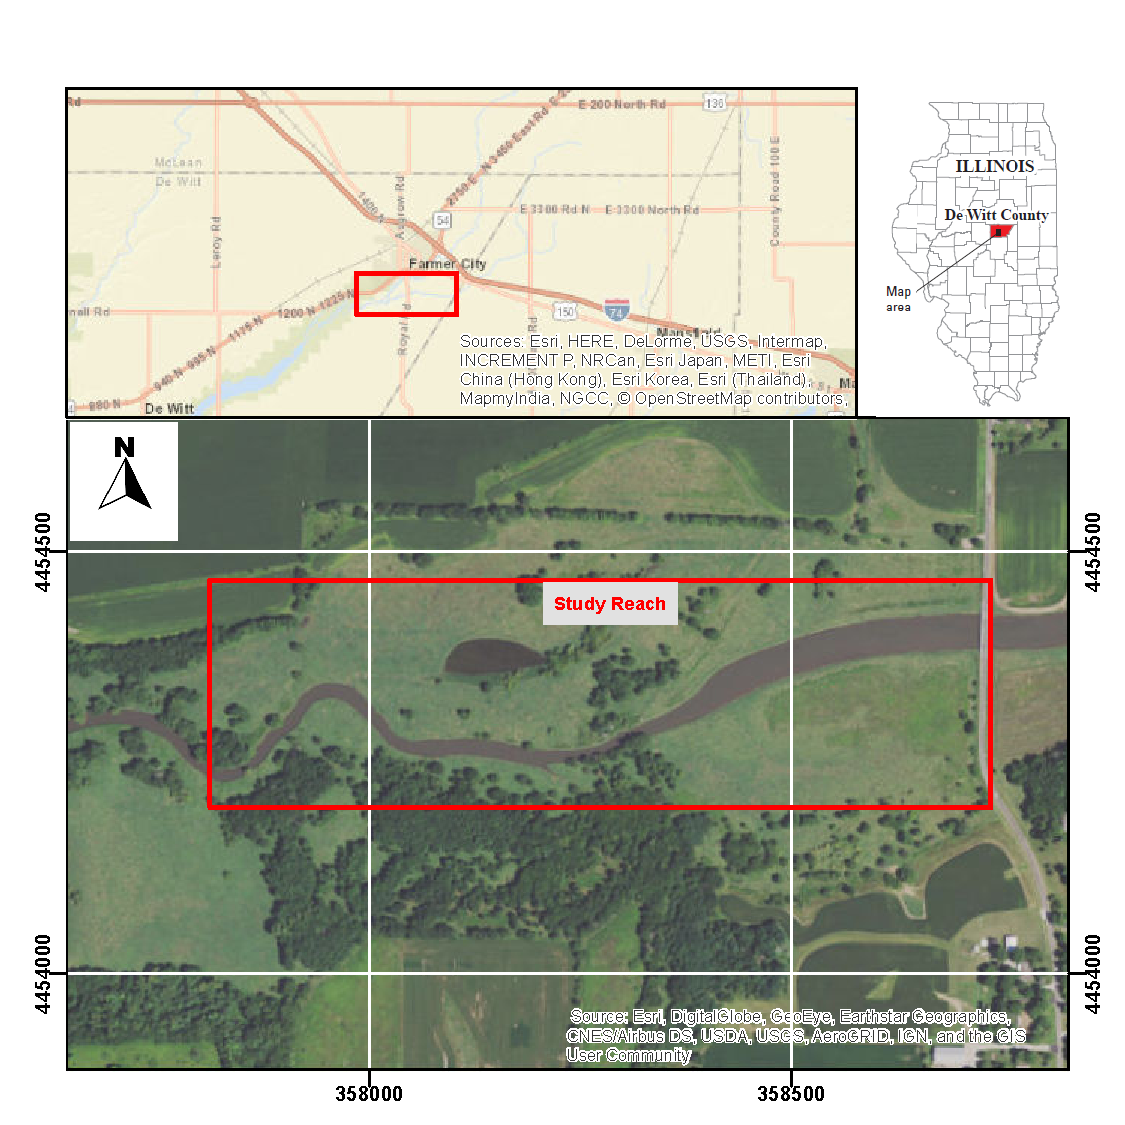
\includegraphics[width=\textwidth]{SiteOverview.pdf}
\caption{Salt Creek Study Reach (UTM Coordinates are shown)}
\label{fig:SiteOverview}
\end{figure}

\section{Data Collection}
ADCP data for this study were collected using three M9 Sontek ADCPs. All of the data were collected in a relatively short period on June 1 and 2, 2016 to ensure constant flow conditions. Two Sontek Argonaut Sidelooker instruments and two In-Situ Level Loggers were installed to monitor flow and confirm steady flow conditions over the ADCP measurement period. The following three ‘types’ of ADCP measurements were collected simultaneously throughout the measurement period.
\begin{itemize}
\item 
Stationary ADCP Data – Stationary data were collected at points along two transects (denoted by tag lines) in the study area. This data were collected by anchoring the boat to a point on the tag line and using a minimum time of 10 minutes (time estimate chosen using guidance from \citeN{Muste:2004b} to account for flow fluctuations and turbulence.
\item Transect ADCP Data – Transect data were collected according to the USGS guidance along the cross sections denoted by tag lines.
\item Longitudinal ADCP Data – longitudinal data were collected for the 1 km study area by completing multiple upstream and downstream passes parallel to the river banks. A variety of transverse positions in the river were chosen for the longitudinal measurement passes
\end{itemize}
Fig.~\ref{fig:MeasurementPaths} shows the boat tracks for the stationary, transect, and longitudinal data during the measurement period.

\begin{figure}
\centering
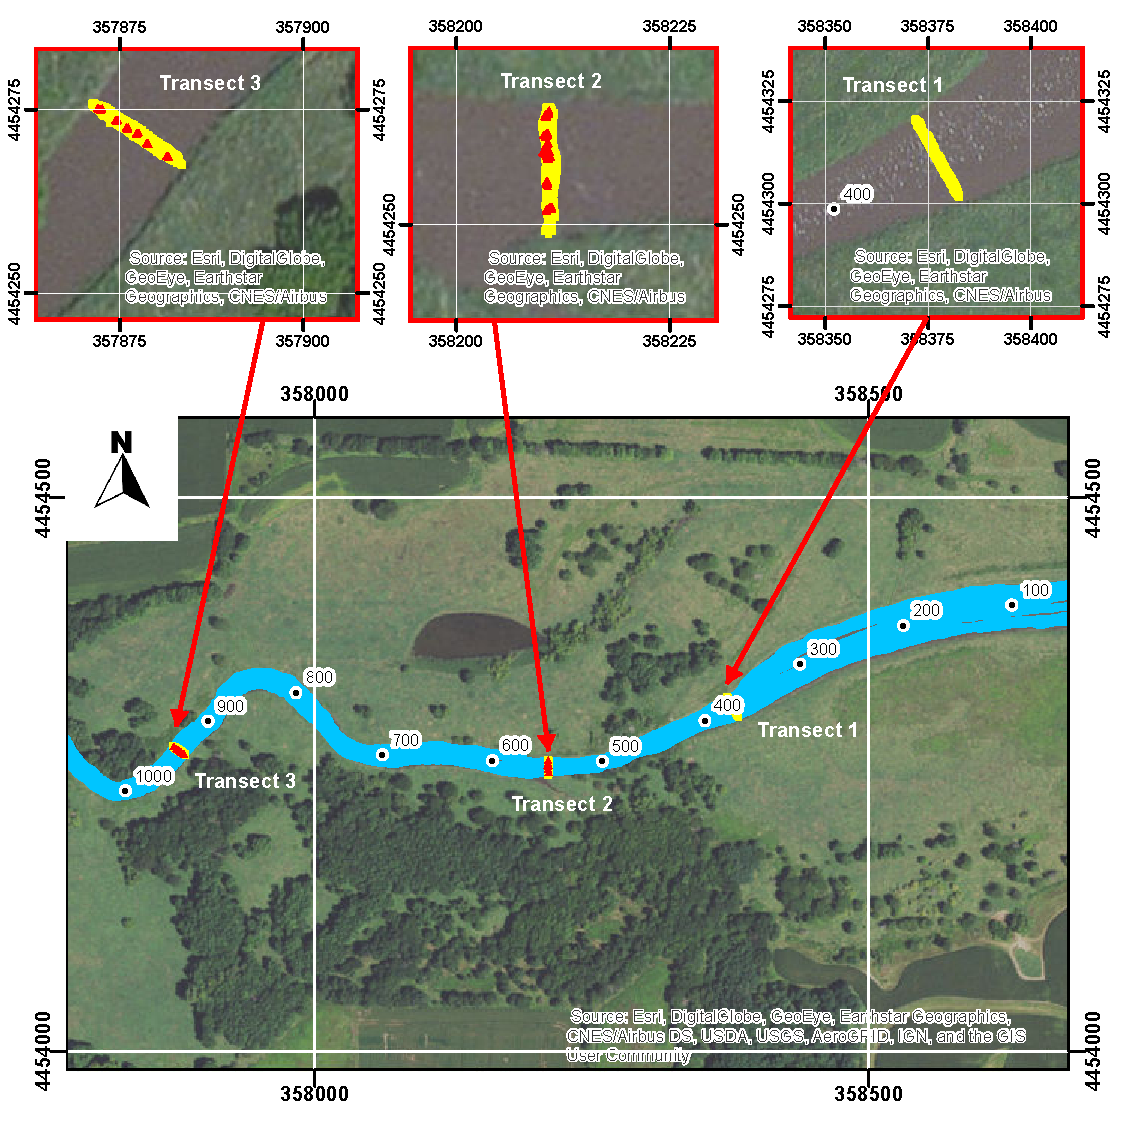
\includegraphics[width=\textwidth]{MeasurementPaths.pdf}
\caption{Measurement Paths: Blue indicates Longitudinal, Yellow indicates Transect, and Red indicates Stationary (UTM Coordinates and River Stations are also shown.)}
\label{fig:MeasurementPaths}
\end{figure}

\section{Methodology}
As mentioned above, ADCP data are typically collected at stationary points or at transects spaced through-out the river. Interpolation methods need to be utilized to estimate the velocity at points located between transects to develop a complete velocity map. \citeN{Kratzer:2006} states that there is very little guidance regarding which interpolation method is best for stream applications such as habitat suitability.

\citeN{Burrough:2015} thoroughly discuss the theory of geographical information systems and the various ways to interpolate data. The following deterministic interpolation approaches were used to interpolate the ADCP velocities in this study: nearest neighbor and inverse distance weighting. In addition, geostatistical interpolation methods including radial basis functions and kriging were investigated.

The interpolation methods chosen for this study were selected considering guidance from bathymetric literature. Since the use of airborne bathymetric LIDAR and other advanced systems on riverine areas became widespread, it has been necessary to incorporate sparsely spread spatial data to develop bathymetric maps for riverine systems. The methodology used to develop bathymetric maps is particularly relevant to creating depth averaged velocity maps. \citeN{Hilldale:2008} and \citeN{Bailly:2010} analyzed rivers that were surveyed using airborne LIDAR collection systems and compared the LIDAR data to surveyed depths along transects. The uncertainty between the LIDAR data and surveyed depths was analyzed to determine the uncertainty in the LIDAR measurements. Uncertainty was presented using typical error statistics including standard deviations and residual analysis. 

\citeN{Glenn:2016} investigated the effect of transect location, spacing, and interpolation on river bathymetry. This study intends on building on the bathymetric related work by performing a similar analysis on river velocities. One main difference between analyzing uncertainty in bathymetric depths and depth averaged velocities is that depths are scalars and depth averaged velocities are two-dimensional vectors. When comparing velocities vectors, one-norm and two-norm methods are discussed in the results section below.

\section{Results}

\subsection{Turbulence}
\citeN{Guerrero:2011} detail a methodology that utilizes the normalized data mean and averaging time to reduce the effect of turbulence on ADCP velocity data. Fig.~\ref{fig:Turbulence} shows the normalized mean variation with respect to averaging time at all of the stationary data collection positions (shown in Fig.~\ref{fig:MeasurementPaths}) located on Transects 2 and 3 for the June 1, data set. The turbulence structure for the area near the transects has a characteristic period (defined as time-averaged velocity within 5\% of 10-minute mean) of approximately 50 to 100 seconds. The average boat velocity for the longitudinal measurements was approximately 0.2 m/s and the transect average boat velocity was approximately 0.1 m/s depending on data collector. Following the guidance presented in \citeN{Guerrero:2011}, the turbulence period and average boat velocity were combined to determine a spatial averaging window of 10 m  for the longitudinal data and 5 m for the transect data. The spatial averaging window was utilized to perform a boxcar average on data collected within a moving 10 m (longitudinal data) and 5 m (transect data) average window. The Velocity Mapping Toolbox (VMT) presented in \citeN{Parsons:2007} also includes a similar averaging window feature. The difference is this study averages using a circular averaging window instead of the anisotropic window presented in the VMT literature. 

\begin{figure}
\centering
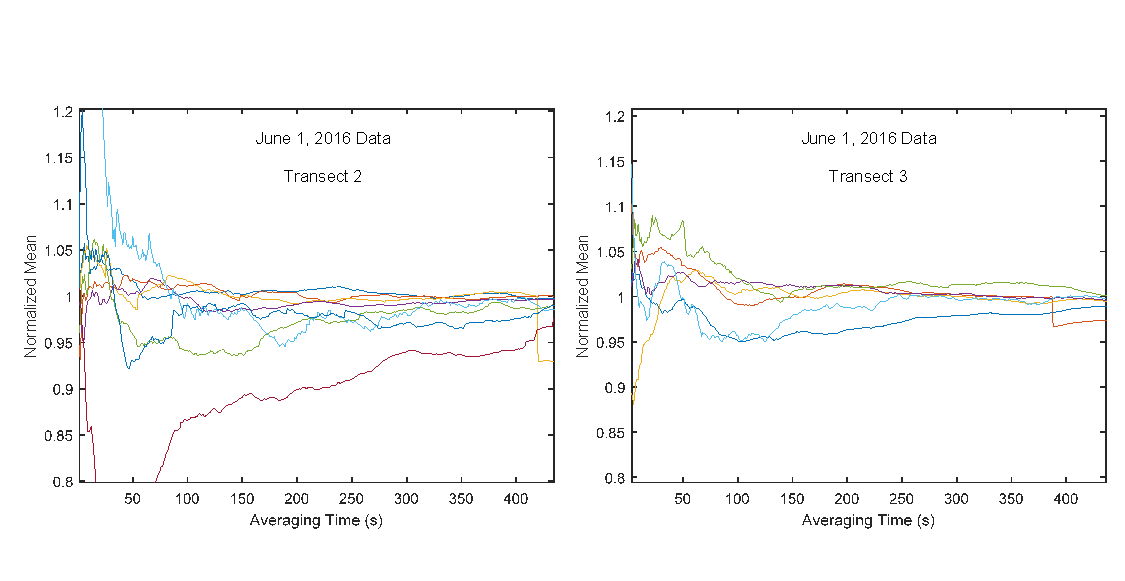
\includegraphics[width=\textwidth]{Turbulence.pdf}
\caption{Plots of Stationary Measurement Data Normalized Mean vs. Average Time (s)}
\label{fig:Turbulence}
\end{figure}

\subsection{Transect Placement and Spacing}
The three transect locations were chosen because of the relatively small curvature of the river at each point, the easy access to the river banks to anchor tag lines, and the absence of pools and riffles in the transect location. The river distance between Transect 1 and 2 is approximately 200 m and the distance between 2 and 3 is 400 m. \citeN{Samuels:1990} recommends that the maximum distance between transects should be no greater than 10 to 20 times of the bankfull width for the development and calibration of one-dimensional hydraulic models. \citeN{Glenn:2016} concludes that the accuracy of bathymetric data derived by interpolating between transects is not significantly dependent on transect location or interpolation method, but is highly correlated to transect spacing. They suggest that transects spaced further apart than 3 times the average bankfull width significantly decreases accuracy in interpolated bathymetric information. In the case of Salt Creek, the bankfull width varies from 21 m at Transect 1 to 17 m at Transect 2 and 15 m at Transect 3; therefore the transect spacing is in line with \citeN{Samuels:1990} recommendation for one-dimensional models but too far apart to satisfy the conclusions presented in \citeN{Glenn:2016}.

\subsection{Coordinate System}
\citeN{Legleiter:2008} explored spatial interpolation of bathymetric data using various kriging methods. In order to account for the anisotropy inherently present in riverine systems, they employed a streamwise coordinate system to aid in interpolation. As described in \citeN{Bailly:2010}, the streamwise direction was determined by defining a centerline, and the direction running perpendicular to the centerline is considered the transverse direction. Fig.~\ref{fig:StreamCoord} illustrates the streamwise/transverse coordinate system for Salt Creek. 

Streams with meanders are particularly susceptible to interpolation errors due to the difference between Euclidean and streamwise distance. Euclidean distance is calculated using the UTM coordinates while streamwise distance is determined using river station and transverse offset distances. Conversely, raw ADCP data are reported in northing and easting coordinates as calculated by the system’s compass and GPS. The combination of the instrument’s default Euclidean coordinate system and the known errors of using Euclidean distance as input into interpolation schemes necessitated an investigation of appropriate coordinate systems for this study.

\begin{figure}
\centering
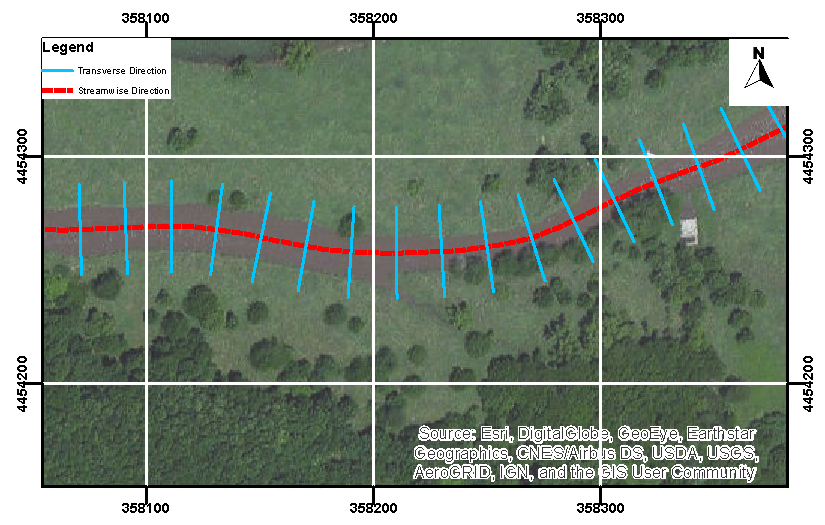
\includegraphics[width=\textwidth]{StreamCoord.pdf}
\caption{Streamwise/Transverse Coordinate System for Salt Creek}
\label{fig:StreamCoord}
\end{figure}

The best section of the river to compare interpolation and data collection methods was just upstream of Transect 1 to just downstream of Transect 2 (River Station (RS) 360 to 560). This section of Salt Creek is relatively straight and devoid of any significant meanders. The area near Transect 3 (RS 930 to 950) was also used for analysis. Velocity interpolations were investigated (the easting and northing vector components were interpolated separately) at points on a uniform grid using northing and easting raw ADCP velocity measurements, ADCP velocities transformed onto a streamwise coordinate system, Euclidean distance, and streamwise calculated distance. For the sections of river described above, the interpolated velocities developed by using the differently transformed data were not significantly different due to the absence of river curvature in the river sections being analyzed. 

For the results described below, velocity vectors at each grid point were interpolated from the north and east components of the ADCP reported velocities. Streamwise coordinate distance was used in the interpolation because the literature advocates this distance is better for reducing error.

\subsection{Interpolated Velocity Maps}
Fig.~\ref{fig:Results360_560} shows the velocity maps generated for the reach from RS 360 (just upstream of Transect 1) to RS 560 (just downstream of Transect 2) using nearest neighbor interpolation and inverse distance interpolation method with a negative exponent of 6. There is a set of plots showing the interpolated data generated using available longitudinal data only and interpolation done using data collected along Transect 1 and 2 only. The June 1 and 2 data shows similar results; therefore, only the June 1 data is presented in the following figures.

\begin{figure}
\centering
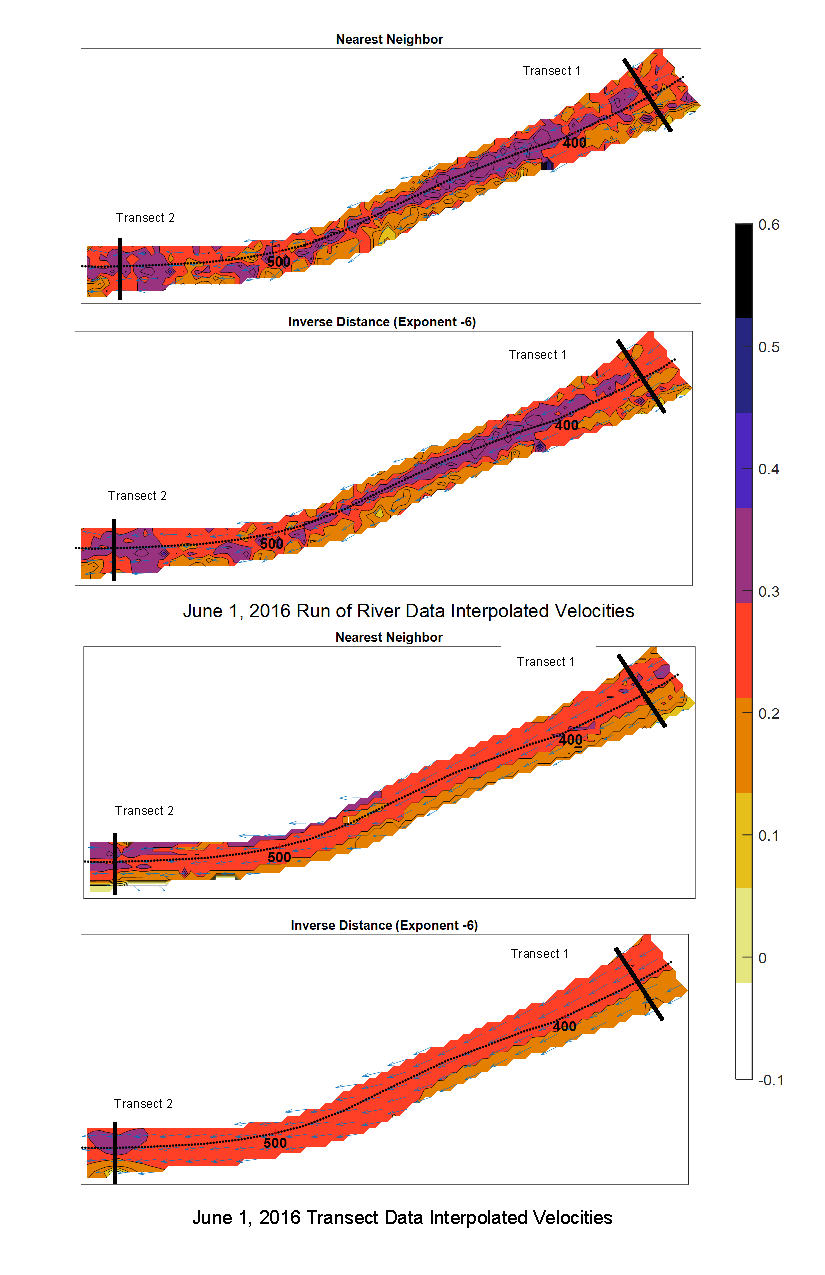
\includegraphics[width=5.3in]{Results360_560.pdf}
\caption{Interpolated Velocities from RS 360 to 560. The colors represent downstream velocity (m/s) and the velocity vectors are shown using the interpolated northing and easting velocity components.}
\label{fig:Results360_560}
\end{figure}

Fig.~\ref{fig:Results360_560} illustrates that the longitudinal data can be used to generate a detailed picture of velocity patterns for Salt Creek. Conversely, the transect data is limited in predicting velocities throughout the 200 m reach. It is possible (and will be investigated below) that the transect data is more accurate in the area very close to the transect location, but Fig.~\ref{fig:Results360_560} illustrates the issues with using this data to interpolate across long distances between transects.

To investigate the precision of interpolated longitudinal versus interpolated transect velocities at each transect location, velocity maps (shown in Figs.~\ref{fig:Results360_380} through ~\ref{fig:Results930_950}) were generated centered on RS 373 (location of Transect 1), RS 550 (location of Transect 2), RS 938 (location of Transect 3). In these figures, the transect data may provide more detailed representation of velocity than the longitudinal data. However, Figs.~\ref{fig:Results360_380}, ~\ref{fig:Results540_560}, and ~\ref{fig:Results930_950} show the longitudinal results qualitatively match the transect data. Another important observation is that the transect interpolated results do not show the lateral velocity variability even in these short reaches (length of 20 m) that the longitudinal results illustrate.

These maps provide a qualitative picture of the different velocities interpolated using the different data types. They also give insight into the difference between interpolation methods. The nearest neighbor method is powerful because it assumes that velocities in a riverine system at any point of interest are going to be most similar to data collected closest to the point of interest. One drawback to the method is that it can amplify the effect of more extreme measurement values. In addition, data points closest to a point of interest may be dissimilar from the point of interest (i.e. points in the thalweg of a channel may be more similar to other further away points in the thalweg versus points near the bank which may be located closer). Inverse distance interpolation will produce similar results to nearest neighbor as the weighting exponent is increased. When the weighting exponent is decreased to zero the interpolated result is the sample mean of the data set, which effectively eliminates any information about spatial differences. 

\begin{figure}
\centering
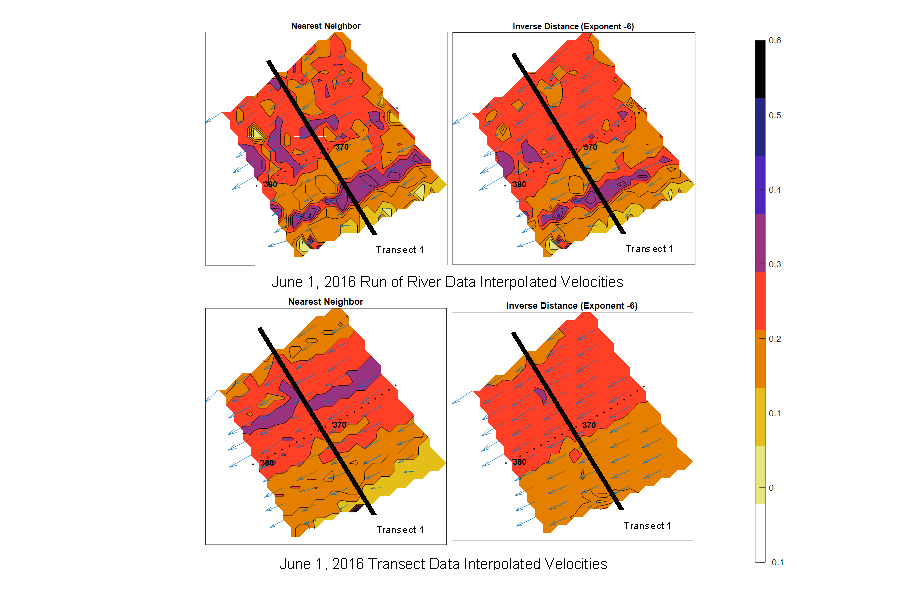
\includegraphics[width=5.5in]{Results360_380.pdf}
\caption{Interpolated Velocities from RS 360 to 380. The colors represent downstream velocity (m/s) and the velocity vectors are shown using the interpolated northing and easting velocity components.}
\label{fig:Results360_380}
\end{figure}

\begin{figure}
\centering
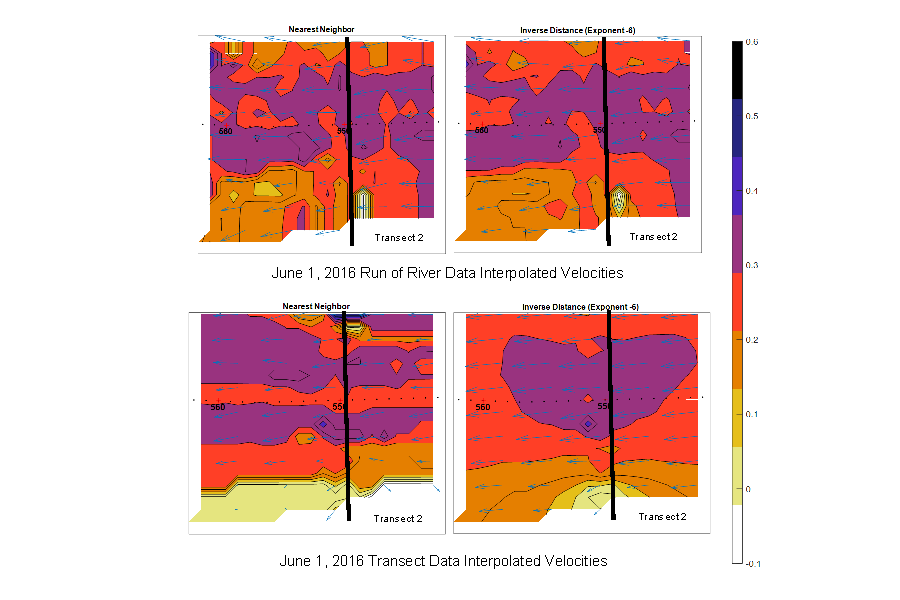
\includegraphics[width=5.5in]{Results540_560.pdf}
\caption{Interpolated Velocities from RS 540 to 560. The colors represent downstream velocity (m/s) and the velocity vectors are shown using the interpolated northing and easting velocity components.}
\label{fig:Results540_560}
\end{figure}

\begin{figure}
\centering
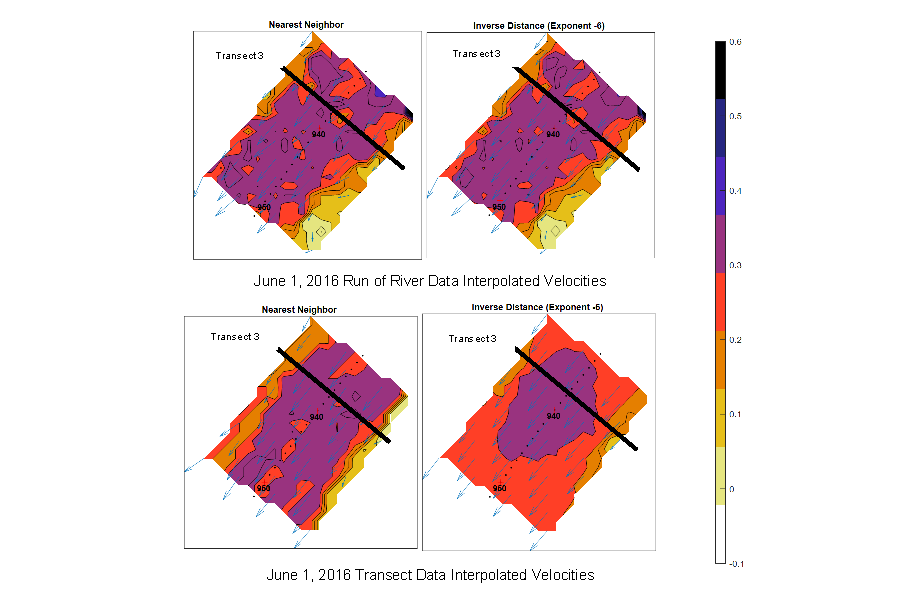
\includegraphics[width=5.5in]{Results930_950.pdf}
\caption{Interpolated Velocities from RS 930 to 950. The colors represent downstream velocity (m/s) and the velocity vectors are shown using the interpolated northing and easting velocity components.}
\label{fig:Results930_950}
\end{figure}

In addition to nearest neighbor and inverse distance interpolation, kriging and radial basis function interpolation methods were investigated. Unfortunately, the Salt Creek data set did not prove to be robust enough for these methods to provide any extra information. The computational effort for kriging and performing a radial basis interpolation on a reasonable sized grid of points for a 200 m long river reach also proved to be limiting. These methods should continue to be investigated as tools for this type of analysis.

The velocity results from various interpolation simulations suggested that an inverse distance method with a medium to large negative exponent, such as 6, produced plausible velocities for the sections of river being analyzed while mitigating some of the inherent drawbacks present in the nearest neighbor method. Thus, the inverse distance weighting method with a negative exponent of 6 will be used for subsequent results and conclusions presented in this study.

\subsection{Velocity Difference Between Data Collection Methods}
Because velocity is a vector rather than a scalar, the difference between interpolation methods and measurement techniques is hard to quantify. A two-norm vector comparison is useful when analyzing northing and easting velocity components. A one-norm vector comparison was useful for comparing the streamwise velocity coordinate. Fig.~\ref{fig:ErrorMap} was generated by calculating the relative error between the longitudinal interpolated and transect streamwise velocities for the inverse distance scheme (negative exponent of 6). For the purpose of this study relative error will be defined by the relationship in Eq.~\ref{eq:Error}:

\begin{equation} \label{eq:Error}
Relative Error =  \lvert \frac{Velocity - TrueVelocity}{TrueVelocity}\rvert\;.
\end{equation}

\begin{figure}
\centering
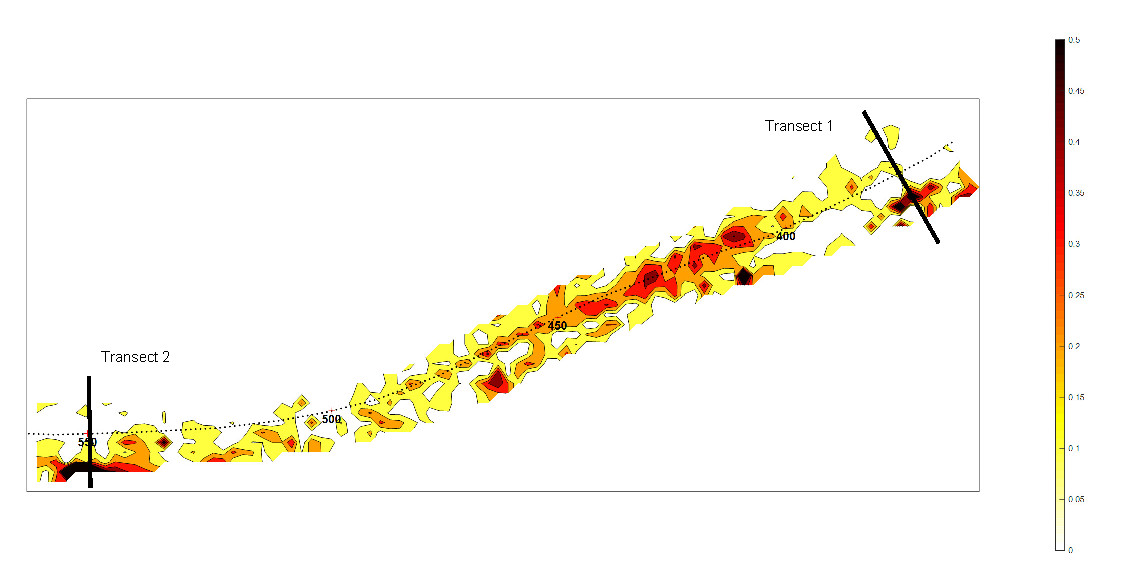
\includegraphics[width=\textwidth]{ErrorMap.pdf}
\caption{Relative Error for Velocity from RS 360 to 560}
\label{fig:ErrorMap}
\end{figure}

The transect interpolated velocities were considered the true velocity in Fig.~\ref{fig:ErrorMap}, although that does not imply (in this case) that the transect velocities are more precise throughout the river reach shown.  Fig.~\ref{fig:ErrorMap} illustrates the generally close agreement between interpolated values generated by each measurement technique near the transect locations (RS 370 and 550) and the increasing disparity as the interpolation location gets further from the transect location. The figure shows relative error greater than 35\% between RS 400 and 450. Note that there are two small areas of higher error at the transect location, which highlights the difference between the higher density of transect collected data and more sparsely collected longitudinal data. It is expected that the transect data is more precise at the transect location and the longitudinal is more precise between transects. More transect data at various transect distance spacings need to be compared to longitudinal data to provide guidance regarding at what distance away from the transect location does the longitudinal method provide more precise results than the transect data collection method.

As explained in Section 6.1, stationary measurement data were collected concurrently with the longitudinal and transect measurements at Transects 2 and 3 to account for the effect of turbulence. The stationary measurements represent time-averaged, depth-averaged, true velocity estimates for specific locations along Transects 2 and 3. Fig.~\ref{fig:ErrorVelocity} shows the difference between the transect and longitudinal interpolations and the time-averaged stationary velocity measurements along Transects 2 and 3. The interpolated velocity difference at each stationary measurement collection point provides a quantitative value to assess the precision of the interpolated velocity estimates.

\begin{figure}
\centering
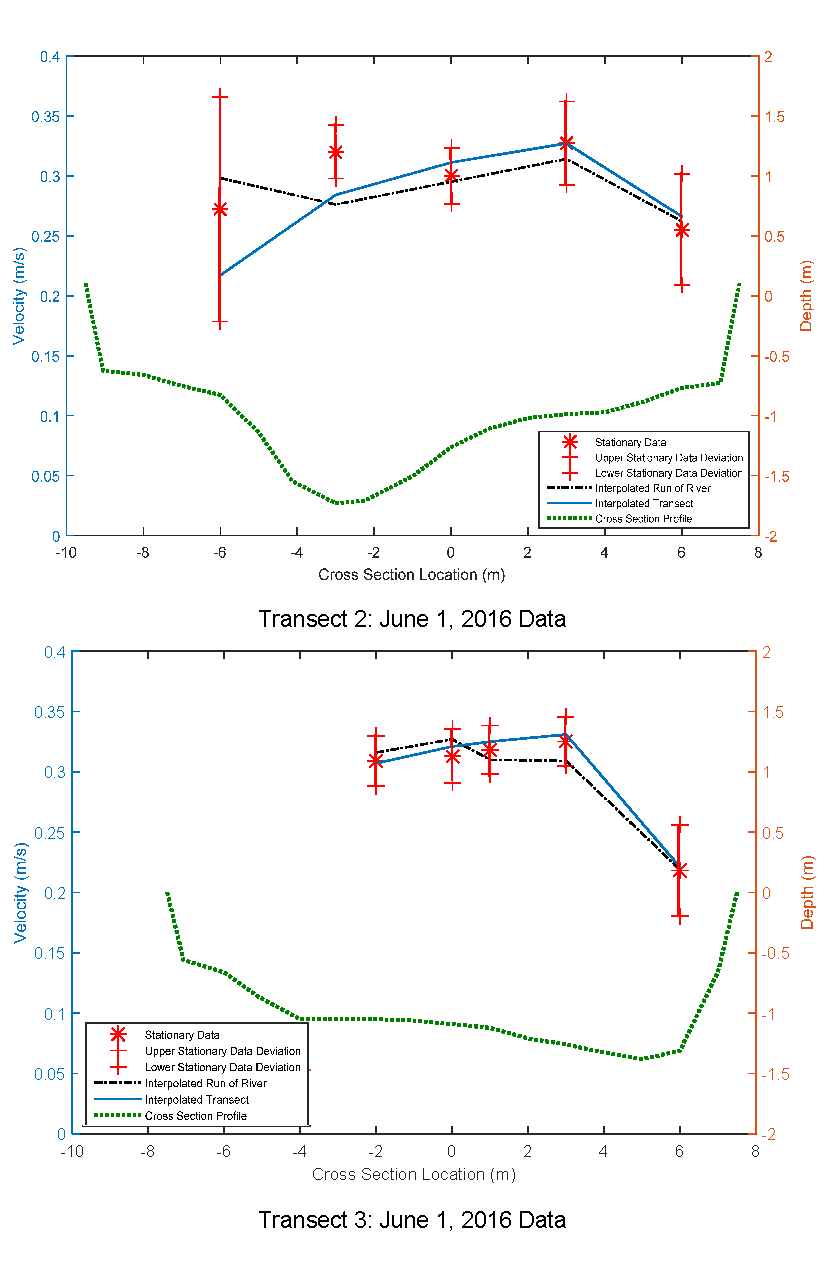
\includegraphics[width=5.2in]{ErrorVelocity.pdf}
\caption{Comparison Between Time Average Stationary Velocity Magnitudes and Interpolated Transect and Longitudinal for June 1, 2016 Data (Whiskers Indicate One Standard Deviation)}
\label{fig:ErrorVelocity}
\end{figure}

\section{Discussion}
\subsection{Velocity Uncertainty}

Using Figs.~\ref{fig:Results360_560}-~\ref{fig:ErrorMap} as qualitative comparison tools, interpolated velocities derived from longitudinal and transect data appear to perform as expected. The two data collection methods are similar in areas near the transect locations, and they diverge significantly in areas further from the transect. As quoted above, \citeN{Glenn:2016} concludes that transect spacing further apart than 3 times the average bankfull width significantly decreases precision in interpolated bathymetric information. The results from Figs.~\ref{fig:Results360_560}-~\ref{fig:ErrorMap} suggest that the transect spacing (significantly larger than 3 times the average bankfull width) used for Salt Creek is too far to precisely interpolate velocities in-between transect locations. The alternative run or river data collection method gives a more detailed picture of the velocities interpolated between transect locations. 

In order to quantitatively assess the data collection methods, the interpolated transect and longitudinal velocities were compared to time-average stationary velocities located on Transects 2 and 3. Fig.~\ref{fig:ErrorVelocity} presents the velocity results and Table~\ref{table:VelocityErr} below presents the error statistics for each stationary measurement point using the inverse distance interpolation method with negative exponent of 6. In Table~\ref{table:VelocityErr}, the time-averaged velocity determined at each stationary point is assumed to be the true velocity value for the error calculations.

\begin{table}
\caption{Comparison Between Time Average Stationary Velocity Magnitudes and Interpolated Transect and Longitudinal}
\label{table:VelocityErr}
\centering
\begin{tabular}{p{2.8cm}p{2cm}p{1.8cm}p{2cm}p{1.8cm}p{2cm}p{2cm}}
\hline\hline
\multicolumn{7}{c}{Transect 2 Location: June 1, 2016 Data} \\
\hline\hline
Offset Measured From River Centerline (m) &
Time-Averaged Stationary Velocity (m/s) &
Interpolated Longitudinal Velocity (m/s)  &
Interpolated Transect Velocity (m/s)  &
Interpolated Longitudinal Relative Error  &
Interpolated Transect Relative Error &
Standard Deviation Stationary Velocity (m/s) \\
\hline
-6	& 0.272	& 0.298 & 0.217 & 9.71\% & 20.03\% & 0.093\\
-3 & 0.320 & 0.276 & 0.284 & 13.88\% & 11.14\% & 0.023\\		
0 & 0.300 & 0.295 & 0.311 & 1.94\% & 3.57\% & 0.023\\		
3 & 0.327 & 0.314 & 0.327 & 4.03\% & 0.03\% & 0.035 \\		
6 &	0.255 & 0.262 & 0.266 & 2.96\% & 4.47\% & 0.047\\
\hline\hline
\multicolumn{7}{c}{Transect 3 Location: June 1, 2016 Data} \\
\hline\hline
-2  & 0.309 & 0.316 & 0.307 & 2.15\% & 0.64\% & 0.021 \\
0 & 0.313 &	0.327 & 0.321 &	4.47\% & 2.85\% & 0.022 \\
1 &	0.318 &	0.310 &	0.325 &	2.38\% & 2.31\% &	0.020 \\
3 &	0.325 &	0.309 &	0.331 &	4.85\% & 1.97\% &	0.020 \\
6 &	0.218 &	0.219 &	0.221 &	0.41\% & 1.22\% &	0.038 \\

\hline\hline
\end{tabular}
\end{table}

From the calculated error shown in Table~\ref{table:VelocityErr}, the root mean squared error (RMSE) for all interpolated transect velocities was 0.0299 and 0.0242 m/s for longitudinal interpolated velocities for Transect 2. The RMSE was 0.0104 for longitudinal and 0.0061 for transect interpolated velocities for Transect 3. The RMSE values indicate that the longitudinal interpolated velocities in this study are almost as precise as the transect interpolated results. It should be noted that the measured velocities in this study are small. Additional analysis should be performed on larger rivers

\subsection{Discharge Uncertainty}
Unlike velocity vectors, discharge is a scalar value that was analyzed for each interpolation method and measurement technique at Transects 1-3. The discharge was calculated following the United States Geological Survey \cite{Mueller:2013} moving boat procedure for calculating discharge at a river cross section by dividing a cross section into vertical sub-sections and taking the vector cross product of the interpolated depth-average velocity (for each measurement technique) and the vector describing the width of the vertical sub-section times the interpolated depth. The interpolated depth was calculated using the same inverse distance interpolation method procedure (as followed with the velocity values) and the ADCP depth measurements collected using both the longitudinal and transect measurement technique.

Table~\ref{table:DischargeErr} shows the comparison between the transect calculated discharge and longitudinal discharge determined from the interpolated longitudinal velocities at RS 370 (Transect 1), RS 550 (Transect 2), and RS 938 (Transect 3). Table~\ref{table:DischargeErr} shows that the relative error between the longitudinal interpolated discharge and the transect calculated discharge is approximately 5\% to 15\% for the June 1 data. The transect calculated discharge represents the true discharge for this relative error calculation, which gives some indication of the uncertainty in using longitudinal measurements to approximate discharge. 

In addition, another prediction of uncertainty is estimating the standard deviation of the discharge at each river station using a first-order second moment variance approximation, which was performed using the interpolated depths and velocities for each measurement technique. The uncertainty values presented in Table~\ref{table:DischargeErr} show that the standard deviation calculated for the longitudinal interpolated discharge are greater than those calculated for the transect interpolated discharge for Transects 1 and 3; it is expected that the transect interpolated discharge should be more precise than longitudinal at the transect locations. Transect 2 appears to be an outlier in the expected behavior of calculated discharge. The important conclusion to draw from the first-order standard deviation approximation is that the longitudinal interpolated discharge compared closely to the transect interpolated discharge for Transects 1 and 3. 

\begin{table}
\caption{Comparison Between Calculated Discharge from Transect and Longitudinal Interpolations (\textit{Std is the 1st-Order 2nd Moment Estimated Standard Deviation})}
\label{table:DischargeErr}
\centering
\begin{tabular}{p{1.3cm}p{1.8cm}p{1.8cm}p{1.8cm}p{2.8cm}p{2.5cm}}
\hline\hline
\multicolumn{6}{c}{June 1, 2016 Data} \\
\hline\hline
River Station (m) &
Interpolated Transect Discharge \(m^{3}/s\) &
Interpolated Longitudinal Discharge \(m^{3}/s\)  &
Longitudinal Relative Error &
Estimated Std Interpolated Transect Discharge \(m^{3}/s\) &
Estimated Std Interpolated Longitudinal Discharge \(m^{3}/s\)\\
\hline
370 & 4.242 & 4.852 & 14.38\% & 0.268 & 0.285\\
550 & 4.864 & 5.339 & 9.76\% & 0.565 & 0.266\\
938 & 4.691 & 4.920 & 4.89\% & 0.350 & 0.398\\

\hline\hline
\end{tabular}
\end{table}

\subsection{Replicate Measurement Effect On Uncertainty}

The relationship between increasing measurement density and decreasing uncertainty in velocity and discharge has been thoroughly investigated in the literature. Fig.~\ref{fig:VelUncertainty} represents the longitudinal interpolated velocity relative error (true velocities are the stationary measurements) in relation to the number of measurement data points used in the interpolation. Only measurement locations within a 10 m radius of the location being interpolated were used for the velocity interpolation. The 10 m radius was chosen to be consistent with the 10 m averaging window (to reduce turbulance), which was described above. Best fit and 95\% confidence lines were used on Fig.~\ref{fig:VelUncertainty} to show the relationship between relative velocity error given number of measurements used for interpolation in a river reach. Transect 2 and 3 data are shown together for this analysis, and the figures are shown according to a non-dimensional channel width distance from the centerline.  

Fig.~\ref{fig:VelUncertainty} serves as a guide for determining the optimal number of longitudinal measurements needed to achieve a desired interpolated velocity precision. For areas near the centerline the benefit of more than 300 measurements is less than for distances 0.1 to 0.2 channel widths away from the centerline. A best fit line was not drawn for channel widths greater than 0.2 because the data showed no correlation between relative error and number of measurements. It is reasonable to expect more variability and less precision near the stream banks. In general, 500 measurements was a good data density to keep relative error less than 5\% in the center 50\% of Salt Creek.

\begin{figure}
\centering
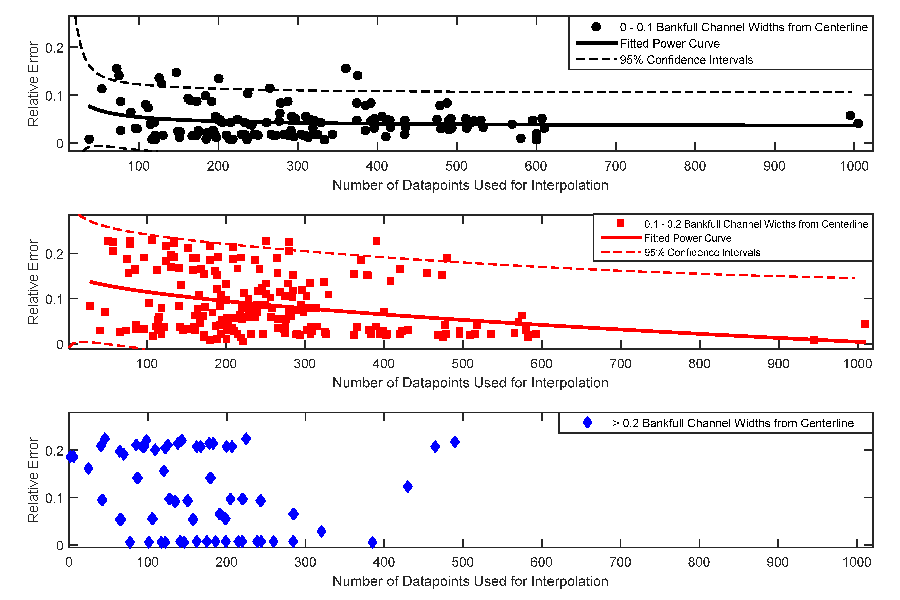
\includegraphics[width=6in]{VelUncertainty.pdf}
\caption{Relative Error of Longitudinal Interpolated Velocities (Compared to Time-Average Stationary Velocities) and Number of Measurements Used in Interpolation}
\label{fig:VelUncertainty}
\end{figure}

\section{Conclusion}
This study builds upon established methods for using ADCPs to measure depth averaged velocity to include a new measurement technique, longitudinal measurements. It has been shown that time averaged stationary measurements reduce velocity uncertainty at a particular location, but are not appropriate for estimating velocities at a river reach scale. Transect measurements are the standard practice for determining velocities over a cross section area. Performing replicate transect measurements reduces the temporal uncertainty and provides velocity information over a larger area; however, it has been shown that the distance between transects is a significant factor when interpolating velocities between transect locations to determine a river reach scale velocity map.

longitudinal measurements provide less velocity information than transect measurements at an individual cross section, but are more effective at estimating depth average velocities for an entire river reach scale (especially when transect data is far apart). This study analyzed ADCP data that was collected concurrently using stationary, transect, and longitudinal collection methods. 

Stationary measurement data were used as true time-averaged velocities at a particular location. They were also utilized to estimate a spatial averaging window to reduce the effect of turbulence on the transect and longitudinal measurements. When longitudinal and transect interpolated velocities were compared to the stationary data (at the stationary measurement location), both longitudinal and transect RMSE uncertainty was 0.0242 and 0.0299 m/s respectively for Transect 2 and 0.0104 and 0.0061 m/s respectively for Transect 3 using the June 1, 2016 data. This implies both measurement types had a similar precision when compared to the stationary data.

Transect and longitudinal interpolated velocities were also compared at the river reach scale. Velocity maps show the significant  differences at locations far from the transect location. The density of longitudinal measurement data was relatively constant throughout the river, so RMSE values should be similar throughout a river reach. Therefore, transect interpolated velocities must be significantly less precise than longitudinal interpolated velocities at areas far from the transect locations to account for the differences in the interpolated velocity maps.

Discharge was also investigated to compare longitudinal and transect interpolated velocities. Using \citeN{Mueller:2013} as guidance, discharge was calculated at each transect location using longitudinal and transect interpolated velocities. In accordance with standard practice, the transect derived discharge was considered the true discharge, and the longitudinal calculated discharge was approximately 5\% to 15\% higher. The standard deviation, also estimated for longitudinal and transect derived discharge, was similar for both measurement techniques.

Finally, replicate transect measurements are performed to reduce discharge uncertainty due turbulence and other factors. Similarly, the number of longitudinal measurement passes was analyzed to recommend a minimum number of measurements required to produce an reasonable relative error for the given application. In general, 500 measurements was a good data density to keep relative error less than 5\% in the center 50\% of Salt Creek.

\section{Acknowledgements}
The authors would like to offer sincere appreciate to Steven Banjavcic of S and S Database Consultants for all of his effort in development of interpolation analysis software. In addition, they would like to thank John Sloat and Diana Krupa of WaterCube and Craig Huhta of One Fish Engineering for the use of ADCP processing and visualization software.

\pagebreak
\bibliography{ascexmpl-new}
%

\end{document}
